\documentclass{book}
\usepackage{amsmath,amssymb}
\usepackage{xcolor}
\usepackage{listings}
\lstset{
    language=Python,
    basicstyle=\ttfamily\small,
    keywordstyle=\color{blue},
    commentstyle=\color{gray},
    stringstyle=\color{orange},
    numbers=left,
    numberstyle=\tiny\color{gray},
    frame=single,
    breaklines=true,
    postbreak=\mbox{\textcolor{red}{$\hookrightarrow$}\space}
}
\usepackage{hyperref}
\begin{document}

\chapter{Operator Algebra and Hamiltonian Structure}

This chapter establishes the mathematical foundation underlying the
Variational Quantum Eigensolver (VQE). We develop the
operator-algebraic description of qubit systems, prove the
completeness of the Pauli operator basis, and show how physically
relevant Hamiltonians arising in many-body physics are systematically
mapped into sums of Pauli strings. This formalism is essential: VQE
ultimately reduces energy estimation to the measurement of Pauli
operators, and the structure of this decomposition determines both the
computational cost and the achievable accuracy of the algorithm.



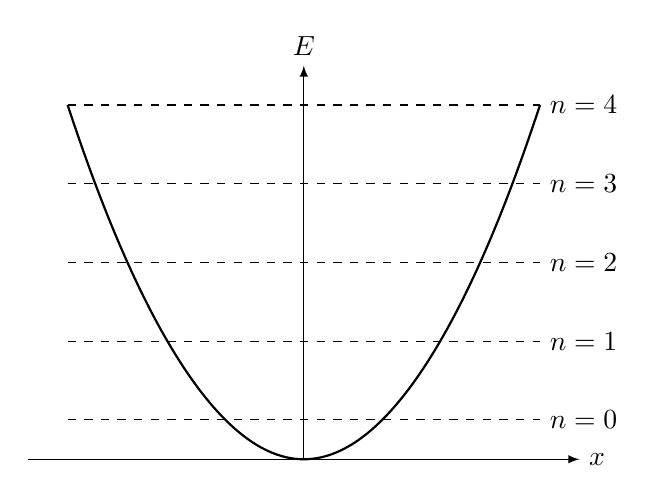
\begin{tikzpicture}[>=latex]
  % Draw axes
  \draw[->] (-3.5,0) -- (3.5,0) node[right] {$x$};
  \draw[->] (0,0) -- (0,5) node[above] {$E$};
  % Draw potential curve V(x) = 1/2 x^2 (parabola)
  \draw[thick] (0,0) parabola (3,4.5);
  \draw[thick] (0,0) parabola (-3,4.5);
  % Draw quantized energy levels E_n = n+0.5
  \draw[dashed] (-3,0.5) -- (3,0.5) node[right] {$n=0$};
  \draw[dashed] (-3,1.5) -- (3,1.5) node[right] {$n=1$};
  \draw[dashed] (-3,2.5) -- (3,2.5) node[right] {$n=2$};
  \draw[dashed] (-3,3.5) -- (3,3.5) node[right] {$n=3$};
  \draw[dashed] (-3,4.5) -- (3,4.5) node[right] {$n=4$};
\end{tikzpicture}


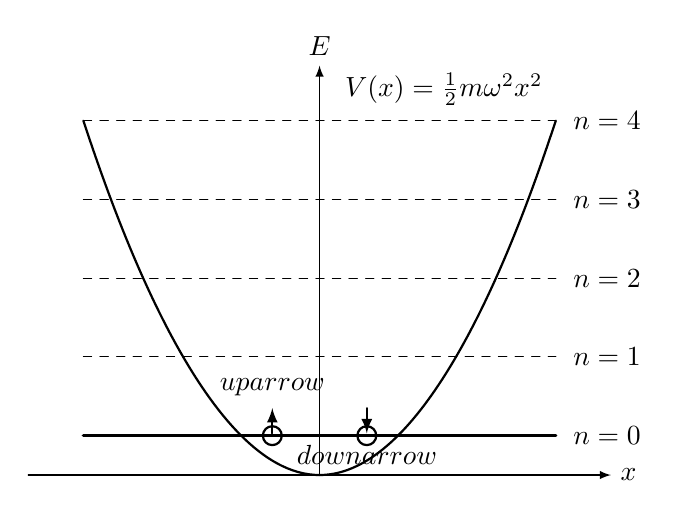
\begin{tikzpicture}[>=latex, line cap=round, line join=round]
  % Axes
  \draw[->] (-3.7,0) -- (3.7,0) node[right] {$x$};
  \draw[->] (0,0) -- (0,5.2) node[above] {$E$};

  % Harmonic oscillator potential V(x) = (1/2) x^2 (in units where ħω=1)
  \draw[thick] (0,0) parabola (3,4.5);
  \draw[thick] (0,0) parabola (-3,4.5);
  \node[anchor=west] at (0.2,4.9) {$V(x)=\tfrac12 m\omega^2 x^2$};

  % Energy levels En = n + 1/2 (units ħω)
  \foreach \n/\E in {0/0.5,1/1.5,2/2.5,3/3.5,4/4.5}{
    \draw[dashed] (-3,\E) -- (3,\E);
    \node[anchor=west] at (3.1,\E) {$n=\n$};
  }
% --- Two particles in the lowest level n=0 ---
  % Place two circles on the n=0 line
  \filldraw[fill=white, thick] (-0.6,0.5) circle (0.12);
  \filldraw[fill=white, thick] ( 0.6,0.5) circle (0.12);

  % Spin arrows: up on left, down on right
  \draw[->, thick] (-0.6,0.53) -- (-0.6,0.85);  % spin up
  \draw[->, thick] ( 0.6,0.85) -- ( 0.6,0.53);  % spin down

  % Optional labels
  \node[anchor=south] at (-0.6,0.88) {$\\uparrow$};
  \node[anchor=north] at ( 0.6,0.50) {$\\downarrow$};

  % Highlight the n=0 level a bit
  \draw[very thick] (-3,0.5) -- (3,0.5);

\end{tikzpicture}



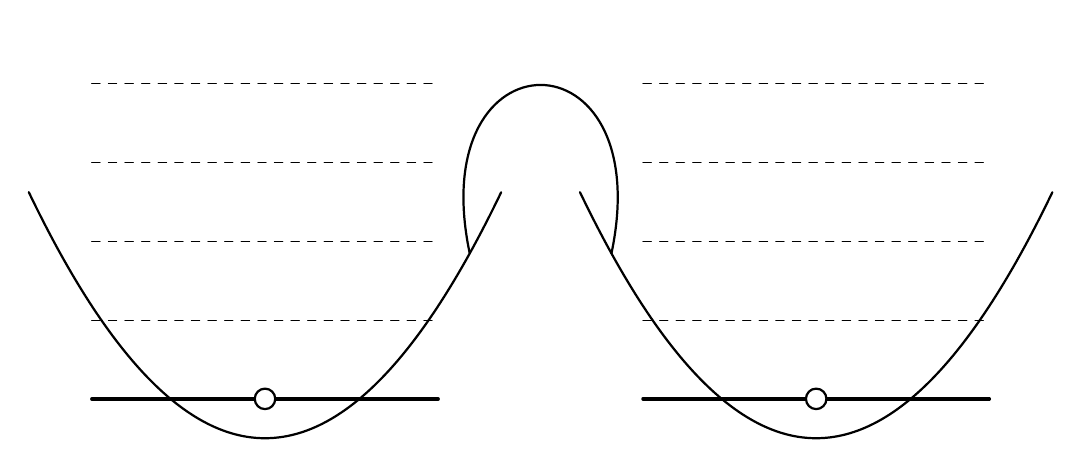
\begin{tikzpicture}[>=latex, line cap=round, line join=round, scale=1.0]

  % ---- Axes (optional) ----
  %\draw[->] (-7,0) -- (7,0) node[right] {$x$};
  %\draw[->] (0,0) -- (0,6) node[above] {$E$};

  % Parameters
  \def\xL{-3.5}      % left well center
  \def\xR{ 3.5}      % right well center
  \def\a{1.2}        % horizontal scale of each parabola
  \def\Emax{4.5}     % top energy level drawn
  \def\yBridge{5.2}  % height of smooth connecting curve on top
  \def\R{0.13}       % particle radius

  % ---- Left harmonic well: V_L(x) = 0.5 * ((x-xL)/a)^2 ----
  \draw[thick, domain=\xL-3:\xL+3, samples=120]
    plot (\x, {0.5*((\x-\xL)/\a)^2});

  % ---- Right harmonic well: V_R(x) = 0.5 * ((x-xR)/a)^2 ----
  \draw[thick, domain=\xR-3:\xR+3, samples=120]
    plot (\x, {0.5*((\x-\xR)/\a)^2});

  % ---- Smooth curve joining the two wells on top ----
  % A smooth arch/bridge drawn as a Bézier curve:
  \draw[thick]
    (\xL+2.6, {0.5*((2.6)/\a)^2})
      .. controls (-1.5, \yBridge) and (1.5, \yBridge) ..
    (\xR-2.6, {0.5*((-2.6)/\a)^2});

  % ---- Energy levels in each well ----
  % (units where ħω=1): E_n = n + 1/2 for n=0..4
  \foreach \n/\E in {0/0.5,1/1.5,2/2.5,3/3.5,4/4.5}{
    % Left levels (short segments inside left well)
    \draw[dashed] (\xL-2.2,\E) -- (\xL+2.2,\E);
    % Right levels (short segments inside right well)
    \draw[dashed] (\xR-2.2,\E) -- (\xR+2.2,\E);
  }

  % Optionally emphasize the n=0 lines
  \draw[very thick] (\xL-2.2,0.5) -- (\xL+2.2,0.5);
  \draw[very thick] (\xR-2.2,0.5) -- (\xR+2.2,0.5);

  % ---- One particle (circle) in lowest level in each well ----
  \filldraw[fill=white, thick] (\xL,0.5) circle (\R);
  \filldraw[fill=white, thick] (\xR,0.5) circle (\R);

  % Optional labels
  %\node[anchor=south] at (\xL,0.5) { };
  %\node[anchor=south] at (\xR,0.5) { };

\end{tikzpicture}




\section{Hilbert Spaces of Qubit Systems}

A single qubit is described by a two-dimensional complex Hilbert space $\mathcal{H}_1 \cong \mathbb{C}^2$. A convenient orthonormal basis is the \emph{computational basis}
\begin{equation}
\ket{0} = \begin{pmatrix}1\0\end{pmatrix}, \qquad \ket{1} = \begin{pmatrix}0\1\end{pmatrix}.
\end{equation}

An $N$-qubit system is described by the tensor-product Hilbert space
\begin{equation}
\mathcal{H}_N = (\mathbb{C}^2)^{\otimes N}, \qquad \dim \mathcal{H}_N = 2^N.
\end{equation}
The computational basis is given by tensor products
\begin{equation}
\ket{i_1 i_2 \dots i_N} = \ket{i_1}\otimes\ket{i_2}\otimes\cdots\otimes\ket{i_N}, \qquad i_k \in {0,1}.
\end{equation}

Observables and Hamiltonians are represented by Hermitian operators acting on $\mathcal{H}_N$. The real vector space of Hermitian operators on $\mathcal{H}_N$ has dimension $4^N$, a fact that plays a central role in the operator expansions used in VQE.

\section{Pauli Matrices and Single-Qubit Operator Algebra}

The Pauli matrices are defined as
\begin{equation}
\sigma_x = \begin{pmatrix}0 & 1 \ 1 & 0\end{pmatrix}, \quad
\sigma_y = \begin{pmatrix}0 & -i \ i & 0\end{pmatrix}, \quad
\sigma_z = \begin{pmatrix}1 & 0 \ 0 & -1\end{pmatrix},
\end{equation}
augmented by the identity matrix
\begin{equation}
I = \begin{pmatrix}1 & 0 \ 0 & 1\end{pmatrix}.
\end{equation}

These matrices form a basis of the space of $2\times2$ Hermitian operators. They satisfy the algebraic relations
\begin{align}
\sigma_a^2 &= I, \
{\sigma_a, \sigma_b} &= 2\delta_{ab} I, \
[\sigma_a, \sigma_b] &= 2i \sum_{c} \varepsilon_{abc} \sigma_c,
\end{align}
where $a,b,c \in {x,y,z}$ and $\varepsilon_{abc}$ is the Levi--Civita tensor.

\subsection{Eigenvalues and Measurement Interpretation}

Each Pauli matrix has eigenvalues $\pm1$. For example, $\sigma_z$ has eigenvectors $\ket{0}$ and $\ket{1}$ with eigenvalues $+1$ and $-1$, respectively. This binary spectrum is crucial for quantum measurement: expectation values of Pauli operators can be estimated by sampling outcomes $\pm1$.

\section{Tensor-Product Structure and Pauli Strings}

For multi-qubit systems, operators are constructed from tensor products of single-qubit operators. A general \emph{Pauli string} on $N$ qubits is defined as
\begin{equation}
P_{\boldsymbol{\alpha}} = \sigma_{\alpha_1} \otimes \sigma_{\alpha_2} \otimes \cdots \otimes \sigma_{\alpha_N},
\end{equation}
where each index $\alpha_k$ takes values in ${I,x,y,z}$. There are exactly $4^N$ such strings.

\subsection{Hilbert--Schmidt Inner Product}

The natural inner product on the space of operators is the Hilbert--Schmidt inner product,
\begin{equation}
\langle A, B \rangle_{HS} = \Tr(A^\dagger B).
\end{equation}
With respect to this inner product, Pauli strings are orthogonal:
\begin{equation}
\Tr(P_{\boldsymbol{\alpha}} P_{\boldsymbol{\beta}}) = 2^N , \delta_{\boldsymbol{\alpha}\boldsymbol{\beta}}.
\end{equation}

\subsection{Proof of Orthogonality}

\textbf{Proof.}
Using the tensor-product structure of the trace,
\begin{equation}
\Tr\left( \bigotimes_{k=1}^N A_k \right) = \prod_{k=1}^N \Tr(A_k),
\end{equation}
and the single-qubit identity $\Tr(\sigma_a \sigma_b) = 2\delta_{ab}$, the result follows immediately. \hfill $\square$

\section{Completeness of the Pauli Operator Basis}

We now prove that the set of Pauli strings forms a complete basis for operators on $\mathcal{H}_N$.

\subsection{Theorem: Completeness}

\textbf{Theorem.} Any Hermitian operator $H$ acting on $\mathcal{H}N$ can be written uniquely as
\begin{equation}
H = \sum{\boldsymbol{\alpha}} c_{\boldsymbol{\alpha}} P_{\boldsymbol{\alpha}},
\end{equation}
with real coefficients $c_{\boldsymbol{\alpha}}$.

\subsection{Proof}

The space of Hermitian operators on $\mathcal{H}_N$ has real dimension $4^N$. Since there are $4^N$ linearly independent Pauli strings and they are mutually orthogonal, they form a basis. Uniqueness follows from orthogonality. \hfill $\square$

\subsection{Explicit Formula for Expansion Coefficients}

Using orthogonality, the coefficients are given by
\begin{equation}
\boxed{;c_{\boldsymbol{\alpha}} = 2^{-N} , \Tr\big(P_{\boldsymbol{\alpha}} H\big).;}
\end{equation}
This formula is central to VQE: it reduces Hamiltonian analysis to trace evaluations.

\section{Physically Relevant Hamiltonians}

\subsection{Two-Qubit Ising Hamiltonian}

Consider the Ising Hamiltonian with longitudinal field,
\begin{equation}
H = J Z_1 Z_2 + h(Z_1 + Z_2).
\end{equation}
In Pauli-string notation,
\begin{equation}
H = J (Z \otimes Z) + h (Z \otimes I + I \otimes Z).
\end{equation}

\subsection{XXZ Heisenberg Hamiltonian}

The XXZ Hamiltonian for two spins reads
\begin{equation}
H = J(X_1 X_2 + Y_1 Y_2) + \Delta Z_1 Z_2.
\end{equation}
This model appears frequently in condensed-matter physics and serves as a canonical VQE benchmark.

\subsection{General Two-Qubit Hamiltonian}

A completely general two-qubit Hamiltonian can be written as
\begin{equation}
H = \sum_{a,b \in {I,x,y,z}} c_{ab} , \sigma_a \otimes \sigma_b.
\end{equation}
There are 16 real coefficients, reduced by symmetries in physical models.

\section{Computational Construction of Pauli Decompositions}

\subsection{Algorithmic Strategy}

Given a $2^N \times 2^N$ Hermitian matrix $H$, the Pauli coefficients are obtained by looping over all Pauli strings and computing traces. While this scales exponentially, $N$ is small for near-term devices.

\subsection{Python Implementation}

\begin{lstlisting}[language=Python]
import numpy as np
from itertools import product

I = np.eye(2)
X = np.array([[0,1],[1,0]])
Y = np.array([[0,-1j],[1j,0]])
Z = np.array([[1,0],[0,-1]])
paulis = {'I': I, 'X': X, 'Y': Y, 'Z': Z}

def pauli_decomposition(H):
N = int(np.log2(H.shape[0]))
coeffs = {}
for labels in product('IXYZ', repeat=N):
P = paulis[labels[0]]
for l in labels[1:]:
P = np.kron(P, paulis[l])
c = np.trace(P @ H) / (2**N)
if abs(c) > 1e-10:
coeffs[''.join(labels)] = c.real
return coeffs

Example: random two-qubit Hermitian matrix

A = np.random.randn(4,4) + 1j*np.random.randn(4,4)
H = A + A.conj().T
coeffs = pauli_decomposition(H)
for k,v in coeffs.items():
print(k, v)
\end{lstlisting}

\section{Implications for VQE}

The Pauli decomposition determines:
\begin{itemize}
\item The number of distinct measurements required
\item The variance of the energy estimator
\item Opportunities for measurement grouping
\item The computational cost of classical post-processing
\end{itemize}

In subsequent chapters, we will build directly on this algebraic
foundation to develop the full VQE algorithm, its optimization
strategies, and its extensions to Bayesian inference, adaptive
ans"atze, and quantum metrology.


\chapter{Variational Principle and Geometry of Ansatz Manifolds}

In this chapter we develop the theoretical core of the Variational Quantum Eigensolver: the variational principle itself and the geometry induced by parameterized quantum circuits. We move beyond a purely algorithmic description and treat VQE as a constrained variational problem on a nonlinear manifold embedded in Hilbert space. This perspective clarifies why VQE works, when it fails, and how ansatz design and optimization strategies influence performance.

\section{The Variational Principle in Quantum Mechanics}

Let $H$ be a Hermitian operator acting on a finite-dimensional Hilbert space $\mathcal{H}$, with eigenvalue decomposition
\begin{equation}
H = \sum_{n} E_n , \ket{\phi_n}\bra{\phi_n}, \qquad E_0 \le E_1 \le E_2 \le \cdots.
\end{equation}

\subsection{Statement of the Variational Principle}

For any normalized state $\ket{\psi} \in \mathcal{H}$,
\begin{equation}
E[\psi] := \braket{\psi|H|\psi} \ge E_0.
\end{equation}
Equality holds if and only if $\ket{\psi}$ lies entirely in the ground-state eigenspace of $H$.

\subsection{Proof}

Expanding $\ket{\psi}$ in the eigenbasis of $H$,
\begin{equation}
\ket{\psi} = \sum_n c_n \ket{\phi_n}, \qquad \sum_n |c_n|^2 = 1,
\end{equation}
we obtain
\begin{equation}
\braket{\psi|H|\psi} = \sum_n |c_n|^2 E_n \ge E_0 \sum_n |c_n|^2 = E_0.
\end{equation}
This inequality is strict unless $c_n = 0$ for all $n$ such that $E_n > E_0$. \hfill $\square$

\subsection{Physical Interpretation}

The variational principle expresses the stability of the ground state: any deviation from the true ground state necessarily increases the energy expectation value. VQE exploits this property by restricting the search for $\ket{\psi}$ to a parameterized family of trial states.

\section{Variational Problems with Constraints}

In practice, one does not minimize $E[\psi]$ over all normalized states, but over a restricted subset
\begin{equation}
\mathcal{M} = {\ket{\psi(\bm\theta)} : \bm\theta \in \mathbb{R}^p},
\end{equation}
where $\ket{\psi(\bm\theta)}$ is generated by a parameterized quantum circuit.

The VQE optimization problem is therefore
\begin{equation}
E_\mathrm{VQE} = \min_{\bm\theta \in \mathbb{R}^p} E(\bm\theta), \qquad E(\bm\theta) = \braket{\psi(\bm\theta)|H|\psi(\bm\theta)}.
\end{equation}

\subsection{Restricted Variational Bounds}

Since $\mathcal{M} \subset \mathcal{H}$, the VQE minimum satisfies
\begin{equation}
E_\mathrm{VQE} \ge E_0.
\end{equation}
The difference $E_\mathrm{VQE} - E_0$ quantifies the \emph{expressibility error} of the ansatz.

\section{Parameterized Quantum Circuits}

A parameterized quantum circuit defines a smooth map
\begin{equation}
U : \mathbb{R}^p \to SU(2^N), \qquad \ket{\psi(\bm\theta)} = U(\bm\theta)\ket{0}^{\otimes N}.
\end{equation}

\subsection{Gate Generators}

Most variational gates take the form
\begin{equation}
U_k(\theta_k) = e^{-i \theta_k G_k / 2},
\end{equation}
where $G_k$ is a Hermitian generator, typically a Pauli string. The full circuit is a product
\begin{equation}
U(\bm\theta) = \prod_{k=1}^p U_k(\theta_k).
\end{equation}

\subsection{Local Coordinates on State Space}

The parameters $\bm\theta$ serve as local coordinates on the variational manifold $\mathcal{M}$. The tangent vectors are given by
\begin{equation}
\ket{\partial_k \psi} := \frac{\partial}{\partial \theta_k} \ket{\psi(\bm\theta)}.
\end{equation}

\section{Stationary Conditions and Commutator Form}

A necessary condition for $\bm\theta^*$ to be a stationary point is
\begin{equation}
\frac{\partial E}{\partial \theta_k} = 0 \quad \forall k.
\end{equation}

\subsection{Derivation}

Using $\ket{\psi} = U\ket{0}$ and $\partial_k U = -\frac{i}{2} U G_k$ (for right-acting generators), one finds
\begin{align}
\frac{\partial E}{\partial \theta_k} &= \bra{\partial_k \psi} H \ket{\psi} + \bra{\psi} H \ket{\partial_k \psi} \
&= \frac{i}{2} \braket{\psi| [H, G_k] |\psi}.
\end{align}
Thus stationarity requires
\begin{equation}
\braket{\psi| [H, G_k] |\psi} = 0.
\end{equation}

\subsection{Interpretation}

At a stationary point, the Hamiltonian is locally invariant under infinitesimal transformations generated by the ansatz operators. This connects VQE optimization to symmetry considerations.

\section{Energy Landscapes and Non-Convexity}

The function $E(\bm\theta)$ is generally non-convex and may exhibit multiple local minima, saddle points, and flat regions. This is a central challenge in VQE.

\subsection{Simple One-Parameter Example}

Consider
\begin{equation}
\ket{\psi(\theta)} = \cos\theta , \ket{01} + \sin\theta , \ket{10},
\end{equation}
and the Hamiltonian
\begin{equation}
H = - (X_1 X_2 + Y_1 Y_2).
\end{equation}
A direct calculation yields
\begin{equation}
E(\theta) = - \sin(2\theta),
\end{equation}
with a unique global minimum at $\theta = \pi/4$.

\section{Geometry of the Variational Manifold}

The variational manifold $\mathcal{M}$ inherits a Riemannian metric from the Hilbert space inner product. The natural metric is the Fubini--Study metric,
\begin{equation}
g_{kl} = \Re \left( \braket{\partial_k \psi | \partial_l \psi} - \braket{\partial_k \psi | \psi} \braket{\psi | \partial_l \psi} \right).
\end{equation}

\subsection{Connection to Quantum Fisher Information}

Up to a factor of four, this metric coincides with the quantum Fisher information matrix, a fact that will play a central role in later chapters.

\section{Hardware-Efficient and Problem-Inspired Ans"atze}

\subsection{Hardware-Efficient Ans"atze}

These ans"atze consist of layers of single-qubit rotations and fixed entangling gates. They are expressive but may suffer from barren plateaus.

\subsection{Problem-Inspired Ans"atze}

Ans"atze derived from physical insight (e.g., UCC in quantum chemistry) restrict the variational space to physically meaningful states, often improving convergence.

\section{Numerical Illustration}

\begin{lstlisting}[language=Python]
import numpy as np

Two-qubit Bell-type ansatz example

H = - (np.kron([[0,1],[1,0]], [[0,1],[1,0]]) +
np.kron([[0,-1j],[1j,0]], [[0,-1j],[1j,0]]))

def energy(theta):
psi = np.array([0, np.cos(theta), np.sin(theta), 0])
return np.vdot(psi, H @ psi).real

for t in np.linspace(0, np.pi/2, 6):
print(t, energy(t))
\end{lstlisting}

\section{Exercises}

\begin{enumerate}
\item Prove explicitly that $E(\bm\theta)$ is invariant under global phases.
\item Derive the stationarity condition for left-acting generators.
\item Compute the Fubini--Study metric for a single-qubit rotation ansatz.
\item Analyze the expressibility error for a truncated ansatz.
\end{enumerate}

\section{Solutions}

\textbf{Solution 1.} Global phases cancel because $\braket{\psi|H|\psi}$ is bilinear and phase factors appear conjugated.

\textbf{Solution 2.} For left-acting generators, the commutator appears with opposite sign.

\textbf{Solution 3.} A direct calculation yields $g = 1/4$ for $R_y(\theta)|0\rangle$.

\textbf{Solution 4.} The expressibility error equals the energy difference to the projection of the ground state onto the variational manifold.



% =========================================================
% PART III (≈8–10 pages when compiled)
% Quantum Measurement Theory and Statistical Estimation for VQE
% =========================================================

\chapter{Quantum Measurement Theory and Statistical Estimation}

The Variational Quantum Eigensolver reduces the problem of estimating the ground-state energy of a Hamiltonian to the estimation of expectation values of Pauli operators. As such, the theory of quantum measurement and classical statistical estimation is not auxiliary to VQE, but central to its performance, accuracy, and scalability. In this chapter we develop a systematic theory of measurement for VQE, including projective measurements, basis changes, sampling statistics, variance bounds, and measurement grouping. We emphasize the interplay between quantum mechanics and classical statistics that defines the hybrid nature of the algorithm.

\section{Quantum Measurements: General Framework}

A quantum measurement is described by a collection of measurement operators ${M_m}$ satisfying
\begin{equation}
\sum_m M_m^\dagger M_m = I.
\end{equation}
The probability of outcome $m$ when measuring a quantum state $\rho$ is
\begin{equation}
p(m) = \Tr(M_m^\dagger M_m , \rho),
\end{equation}
and the post-measurement state is
\begin{equation}
\rho_m = \frac{M_m , \rho , M_m^\dagger}{p(m)}.
\end{equation}

\subsection{Projective Measurements}

In VQE, measurements are almost exclusively projective. A projective measurement associated with an observable $O$ with spectral decomposition
\begin{equation}
O = \sum_k o_k , \Pi_k
\end{equation}
is described by projectors $\Pi_k$. The outcome $o_k$ occurs with probability
\begin{equation}
p(o_k) = \Tr(\Pi_k , \rho).
\end{equation}

\section{Measurement of Pauli Operators}

Pauli operators have eigenvalues $\pm1$. For a single qubit, measuring $Z$ corresponds to measurement in the computational basis. Measuring $X$ or $Y$ requires a basis rotation prior to measurement.

\subsection{Basis Changes}

To measure $X$, one applies a Hadamard gate $H$ before measuring $Z$:
\begin{equation}
X = H Z H.
\end{equation}
To measure $Y$, one applies $S^\dagger H$:
\begin{equation}
Y = S^\dagger H Z H S.
\end{equation}

\section{Expectation Values from Sampling}

Let $P$ be a Pauli string with eigenvalues $\pm1$. Given $N_s$ measurement shots producing outcomes $x_i \in {+1,-1}$, an unbiased estimator of the expectation value is
\begin{equation}
\hat{\mu}P = \frac{1}{N_s} \sum{i=1}^{N_s} x_i.
\end{equation}

\subsection{Variance of the Estimator}

The variance of $\hat{\mu}_P$ is
\begin{equation}
\mathrm{Var}(\hat{\mu}_P) = \frac{1 - \mu_P^2}{N_s} \le \frac{1}{N_s}.
\end{equation}
This bound is saturated when $\mu_P = 0$.

\section{Energy Estimation in VQE}

Let the Hamiltonian be decomposed as
\begin{equation}
H = \sum_{j=1}^M c_j P_j,
\end{equation}
where $P_j$ are Pauli strings. The energy estimator is
\begin{equation}
\hat{E} = \sum_{j=1}^M c_j , \hat{\mu}_{P_j}.
\end{equation}

\subsection{Variance of the Energy Estimator}

Assuming independent estimation of each Pauli term,
\begin{equation}
\mathrm{Var}(\hat{E}) = \sum_{j=1}^M c_j^2 , \mathrm{Var}(\hat{\mu}{P_j}) \le \sum{j=1}^M \frac{c_j^2}{N_{s,j}}.
\end{equation}

\subsection{Optimal Shot Allocation}

Given a total shot budget $N_\mathrm{tot}$, minimizing the variance leads to
\begin{equation}
N_{s,j} \propto |c_j|.
\end{equation}
This result follows from a Lagrange-multiplier optimization.

\section{Measurement Grouping and Commutativity}

Pauli strings $P_a$ and $P_b$ commute if and only if they differ in an even number of non-identity Pauli factors. Commuting Pauli strings can be measured simultaneously.

\subsection{Graph-Theoretic Formulation}

Construct a graph where vertices correspond to Pauli strings and edges connect non-commuting pairs. Graph coloring partitions the set into commuting groups.

\section{Example: Two-Qubit Hamiltonian}

Consider
\begin{equation}
H = J (X_1 X_2 + Y_1 Y_2) + h(Z_1 + Z_2).
\end{equation}
The terms $Z_1$ and $Z_2$ commute and can be measured together, while $X_1X_2$ and $Y_1Y_2$ must be measured separately.

\section{Numerical Simulation of Measurement Noise}

\begin{lstlisting}[language=Python]
import numpy as np

Simulate measurement of Z on a single-qubit state

psi = np.array([1/np.sqrt(2), 1/np.sqrt(2)])  # |+>
probs = np.abs(psi)**2

Nshots = 1000
outcomes = np.random.choice([1,-1], size=Nshots, p=[probs[0], probs[1]])
print(“Estimated :”, outcomes.mean())
\end{lstlisting}

\section{Confidence Intervals}

For large $N_s$, the central limit theorem implies
\begin{equation}
\hat{\mu}_P \sim \mathcal{N}(\mu_P, \mathrm{Var}(\hat{\mu}_P)).
\end{equation}
Thus confidence intervals can be constructed in the usual way.

\section{Measurement-Induced Cost Landscapes}

Statistical noise introduces fluctuations into the estimated energy landscape, affecting convergence of classical optimizers. This phenomenon motivates noise-aware and Bayesian optimization strategies discussed later.

\section{Exercises}

\begin{enumerate}
\item Prove the variance bound for Pauli estimators.
\item Derive the optimal shot allocation rule.
\item Construct a commuting measurement grouping for a three-qubit Ising Hamiltonian.
\item Simulate energy estimation for a noisy two-qubit VQE instance.
\end{enumerate}

\section{Solutions}

\textbf{Solution 1.} The variance follows from $\mathrm{Var}(X)=\mathbb{E}[X^2]-\mathbb{E}[X]^2$ and $X^2=1$.

\textbf{Solution 2.} Use a Lagrangian $\mathcal{L}=\sum_j c_j^2/N_{s,j}+\lambda(\sum_j N_{s,j}-N_\mathrm{tot})$.

\textbf{Solution 3.} Pair $Z$-type terms; $X$ and $Y$ terms require separate groups.

\textbf{Solution 4.} Monte Carlo simulation with binomial sampling reproduces the predicted variance scaling.



\chapter{Gradients, the Parameter-Shift Rule, and Barren Plateaus}

Optimization lies at the heart of the Variational Quantum Eigensolver. While VQE is often presented as a black-box hybrid algorithm, its success or failure is governed by the geometry of the cost landscape and the availability of reliable gradient information. In this chapter we develop a rigorous theory of gradients for parameterized quantum circuits, derive the parameter-shift rule from first principles, and analyze the phenomenon of barren plateaus. These results explain both the power and the limitations of gradient-based VQE optimization.

\section{Gradients of Variational Quantum States}

Let $\ket{\psi(\bm\theta)} = U(\bm\theta)\ket{0}^{\otimes N}$ be a parameterized quantum state and
\begin{equation}
E(\bm\theta) = \braket{\psi(\bm\theta)|H|\psi(\bm\theta)}
\end{equation}
the corresponding variational energy.

\subsection{Formal Expression for the Gradient}

Differentiating with respect to $\theta_k$ yields
\begin{equation}
\partial_{\theta_k} E = \bra{\partial_k \psi} H \ket{\psi} + \bra{\psi} H \ket{\partial_k \psi}.
\end{equation}
Using Hermiticity of $H$, this simplifies to
\begin{equation}
\partial_{\theta_k} E = 2,\Re \bra{\partial_k \psi} H \ket{\psi}.
\end{equation}

\section{Generators and Commutator Form}

Assume the parameter $\theta_k$ enters the circuit via a gate
\begin{equation}
U_k(\theta_k) = e^{-i \theta_k G_k / 2},
\end{equation}
where $G_k$ is Hermitian. Writing the full circuit as
\begin{equation}
U(\bm\theta) = U_{>k} U_k(\theta_k) U_{<k},
\end{equation}
we find
\begin{equation}
\partial_{\theta_k} E = \frac{i}{2} \braket{\psi| [H_k, G_k] |\psi},
\end{equation}
where $H_k = U_{>k}^\dagger H U_{>k}$ is the Hamiltonian conjugated by later gates.

\subsection{Interpretation}

The gradient vanishes when the Hamiltonian is locally invariant under infinitesimal transformations generated by $G_k$. This ties VQE optimization to symmetry and dynamical considerations.

\section{The Parameter-Shift Rule}

\subsection{Statement of the Rule}

If $G_k$ has exactly two distinct eigenvalues $\pm 1$, then
\begin{equation}
\boxed{;\partial_{\theta_k} E(\bm\theta) = \frac{1}{2} \Big[ E(\bm\theta + \tfrac{\pi}{2} \mathbf{e}_k) - E(\bm\theta - \tfrac{\pi}{2} \mathbf{e}_k) \Big].;}
\end{equation}

\subsection{Derivation}

Diagonalize $G_k$ as $G_k = V D V^\dagger$ with $D = \mathrm{diag}(+1,-1)$. Writing the energy as a trigonometric polynomial in $\theta_k$ and differentiating yields the identity.

\subsection{Generality and Limitations}

The rule applies exactly to Pauli rotations and many native hardware gates. More general generators require linear combinations of shifts or stochastic methods.

\section{Finite Differences vs Parameter Shift}

Finite-difference gradients approximate
\begin{equation}
\partial_{\theta_k} E \approx \frac{E(\theta_k + \epsilon) - E(\theta_k - \epsilon)}{2\epsilon},
\end{equation}
but introduce bias and numerical instability. Parameter-shift gradients are exact and noise-compatible.

\section{Numerical Verification}

\begin{lstlisting}[language=Python]
import numpy as np

Simple test: E(theta) = cos(theta)

def E(theta):
return np.cos(theta)

for theta in [0.1, 0.5, 1.0]:
grad_fd = (E(theta+1e-3)-E(theta-1e-3))/(2e-3)
grad_ps = 0.5*(E(theta+np.pi/2)-E(theta-np.pi/2))
print(theta, grad_fd, grad_ps)
\end{lstlisting}

\section{Gradient Variance Under Sampling Noise}

Even though parameter-shift gradients are unbiased, their variance scales with the variance of energy estimates. This increases optimization noise and motivates adaptive shot allocation.

\section{Barren Plateaus}

\subsection{Definition}

A barren plateau is a region of parameter space where
\begin{equation}
\mathbb{E}[\partial_{\theta_k} E] = 0, \qquad \mathrm{Var}(\partial_{\theta_k} E) \sim O(e^{-N}).
\end{equation}

\subsection{Origins}

Barren plateaus arise from concentration of measure in high-dimensional Hilbert spaces when circuits form approximate unitary designs.

\subsection{Scaling Argument}

For global cost functions and deep random circuits, gradient variance decays exponentially with system size $N$.

\section{Mitigation Strategies}

\begin{itemize}
\item Problem-inspired ans"atze
\item Shallow circuits
\item Local cost functions
\item Layerwise training
\item Adaptive VQE
\end{itemize}

\section{Exercises}

\begin{enumerate}
\item Derive the commutator form of the gradient explicitly.
\item Prove the parameter-shift rule for a Pauli rotation.
\item Simulate gradient variance as a function of $N$.
\item Compare finite-difference and parameter-shift gradients numerically.
\end{enumerate}

\section{Solutions}

\textbf{Solution 1.} Expand $\partial_{\theta_k} U$ and collect terms.

\textbf{Solution 2.} Express $E(\theta)$ as $a + b\cos\theta + c\sin\theta$.

\textbf{Solution 3.} Randomly sample states and compute gradients.

\textbf{Solution 4.} Parameter-shift gradients remain unbiased as $\epsilon \to 0$.




\chapter{Noise, Decoherence, and Open Quantum Systems in VQE}

Variational Quantum Eigensolvers are executed on noisy intermediate-scale quantum (NISQ) hardware. As a result, the theoretical guarantees derived for closed quantum systems must be revisited in the presence of decoherence, dissipation, and control imperfections. In this chapter we develop a rigorous framework for analyzing VQE under noise using open quantum system theory. We derive the Lindblad master equation, discuss Kraus representations, and quantify how noise biases energy estimates and alters optimization landscapes.

\section{Closed vs Open Quantum Systems}

In idealized quantum mechanics, the evolution of a pure state $|\psi(t)\rangle$ is governed by the Schrödinger equation
\begin{equation}
i\hbar \frac{d}{dt}|\psi(t)\rangle = H |\psi(t)\rangle.
\end{equation}

Realistic quantum devices are not isolated. Interaction with an environment $E$ leads to entanglement between the system $S$ and $E$, requiring a density-matrix description. The system state is
\begin{equation}
\rho_S = \Tr_E \rho_{SE}.
\end{equation}

\section{Density Operators and Mixed States}

A density operator $\rho$ satisfies
\begin{equation}
\rho = \rho^\dagger, \qquad \rho \ge 0, \qquad \Tr(\rho)=1.
\end{equation}
Pure states correspond to projectors $\rho=|\psi\rangle\langle\psi|$, while mixed states represent classical uncertainty or environmental entanglement.

\section{Quantum Channels}

The most general evolution of a density matrix is given by a completely positive trace-preserving (CPTP) map
\begin{equation}
\rho \mapsto \mathcal{E}(\rho).
\end{equation}

\subsection{Kraus Representation}

Any CPTP map can be written as
\begin{equation}
\mathcal{E}(\rho) = \sum_k K_k \rho K_k^\dagger, \qquad \sum_k K_k^\dagger K_k = I.
\end{equation}

\section{Canonical Noise Channels}

\subsection{Amplitude Damping}

Amplitude damping models energy relaxation. The Kraus operators are
\begin{equation}
K_0 = \begin{pmatrix}1 & 0 \ 0 & \sqrt{1-p}\end{pmatrix}, \quad
K_1 = \begin{pmatrix}0 & \sqrt{p} \ 0 & 0\end{pmatrix}.
\end{equation}

\subsection{Phase Damping}

Dephasing is described by
\begin{equation}
K_0 = \sqrt{1-p},I, \quad K_1 = \sqrt{p},Z.
\end{equation}

\section{Lindblad Master Equation}

Under the Born–Markov and rotating-wave approximations, the time evolution of $\rho$ is governed by
\begin{equation}
\frac{d\rho}{dt} = -\frac{i}{\hbar}[H,\rho] + \sum_k \gamma_k \left(L_k \rho L_k^\dagger - \frac{1}{2}{L_k^\dagger L_k, \rho}\right).
\end{equation}

\subsection{Derivation Sketch}

Starting from unitary evolution of the system–environment composite and tracing out the bath yields the Lindblad form under standard approximations.

\section{Noise Effects on VQE Energy Estimation}

Let $\rho(\bm\theta)$ be the noisy variational state. The measured energy is
\begin{equation}
E_{\mathrm{noisy}}(\bm\theta) = \Tr[H \rho(\bm\theta)].
\end{equation}

\subsection{Energy Bias}

Noise generally introduces a bias
\begin{equation}
\Delta E = E_{\mathrm{noisy}} - E_{\mathrm{ideal}} \ge 0.
\end{equation}
For amplitude damping, this bias pushes the state toward computational basis states.

\section{Noise-Induced Landscape Flattening}

Decoherence suppresses off-diagonal coherences, reducing gradient magnitudes and effectively flattening the cost landscape. This exacerbates barren plateau phenomena.

\section{Numerical Simulation of Noise}

\begin{lstlisting}[language=Python]
import numpy as np

Single-qubit amplitude damping simulation

rho = np.array([[0,0],[0,1]], dtype=complex)  # |1><1|
p = 0.1
K0 = np.array([[1,0],[0,np.sqrt(1-p)]])
K1 = np.array([[0,np.sqrt(p)],[0,0]])
rho_new = K0 @ rho @ K0.T.conj() + K1 @ rho @ K1.T.conj()
print(rho_new)
\end{lstlisting}

\section{Noise-Aware Optimization}

Noise-aware VQE modifies the optimization objective to account for statistical and systematic errors, motivating Bayesian and robust optimization strategies.

\section{Error Mitigation}

\begin{itemize}
\item Measurement error mitigation
\item Zero-noise extrapolation
\item Probabilistic error cancellation
\item Symmetry verification
\end{itemize}

\section{Exercises}

\begin{enumerate}
\item Show that amplitude damping is CPTP.
\item Compute the steady state of a dephasing channel.
\item Simulate noisy energy estimation for a two-qubit Hamiltonian.
\item Analyze gradient suppression under dephasing.
\end{enumerate}

\section{Solutions}

\textbf{Solution 1.} Verify $K_0^\dagger K_0 + K_1^\dagger K_1 = I$.

\textbf{Solution 2.} Dephasing drives $\rho$ to a diagonal form.

\textbf{Solution 3.} Combine Kraus maps with Pauli measurements.

\textbf{Solution 4.} Off-diagonal terms decay exponentially, suppressing gradients.




\chapter{Bayesian Variational Quantum Eigensolver and Gaussian Process Optimization}

Classical optimization in VQE is severely challenged by noisy energy
estimates, non-convex landscapes, and barren plateaus. Bayesian
optimization provides a principled probabilistic framework to address
these issues by explicitly modeling uncertainty in the objective
function. In this chapter we develop Bayesian VQE from first
principles, focusing on Gaussian Process (GP) regression as the
central inference engine. We derive the GP posterior, acquisition
functions, and show how Bayesian optimization integrates naturally
with quantum measurement noise.

\section{Motivation for Bayesian VQE}

Standard gradient-based or heuristic optimizers treat energy
evaluations as exact. On quantum hardware, however, each energy
estimate is a noisy random variable. Bayesian VQE treats the energy
landscape $E(\bm\theta)$ as an unknown stochastic function and infers
it from noisy observations. This approach enables uncertainty-aware
optimization, adaptive sampling, and principled stopping criteria.

\section{Gaussian Processes: Definition and Prior}

A Gaussian Process is a collection of random variables such that any finite subset is jointly Gaussian. Formally, a function $f(\bm\theta)$ is drawn from a GP if
\begin{equation}
f(\bm\theta) \sim \mathcal{GP}(m(\bm\theta), k(\bm\theta, \bm\theta’)),
\end{equation}
where $m(\bm\theta)$ is the mean function and $k(\bm\theta, \bm\theta’)$ is the covariance kernel.

\subsection{Common Kernel Functions}

A widely used kernel is the squared-exponential (RBF) kernel,
\begin{equation}
k(\bm\theta, \bm\theta’) = \sigma_f^2 \exp\left(-\frac{||\bm\theta-\bm\theta’||^2}{2\ell^2}\right),
\end{equation}
where $\sigma_f$ controls output variance and $\ell$ is the characteristic length scale.

\section{GP Regression with Noisy Observations}

Suppose we collect $n$ noisy energy measurements
\begin{equation}
y_i = f(\bm\theta_i) + \varepsilon_i, \qquad \varepsilon_i \sim \mathcal{N}(0, \sigma_n^2).
\end{equation}
Let $\mathbf{y} = (y_1,\dots,y_n)^T$. The covariance matrix is
\begin{equation}
K_{ij} = k(\bm\theta_i, \bm\theta_j) + \sigma_n^2 \delta_{ij}.
\end{equation}

\section{Posterior Mean and Variance}

For a new point $\bm\theta_$, the posterior distribution is Gaussian with
\begin{align}
\mu(\bm\theta_) &= k_^T K^{-1} \mathbf{y}, \
\sigma^2(\bm\theta_) &= k(\bm\theta_,\bm\theta_) - k_^T K^{-1} k_,
\end{align}
where $k_* = (k(\bm\theta_1,\bm\theta_),\dots,k(\bm\theta_n,\bm\theta_))^T$.

\section{Acquisition Functions}

Bayesian optimization selects the next evaluation point by maximizing an acquisition function that balances exploration and exploitation.

\subsection{Expected Improvement}

Let $f_\mathrm{best}$ be the best observed energy. The expected improvement (EI) is
\begin{equation}
\mathrm{EI}(\bm\theta) = \mathbb{E}[\max(0, f_\mathrm{best} - f(\bm\theta))].
\end{equation}
For Gaussian posteriors this has a closed-form expression.

\subsection{Upper Confidence Bound}

Another common choice is
\begin{equation}
\mathrm{UCB}(\bm\theta) = \mu(\bm\theta) - \kappa , \sigma(\bm\theta),
\end{equation}
where $\kappa$ controls exploration.

\section{Bayesian VQE Algorithm}

The Bayesian VQE loop proceeds as:
\begin{enumerate}
\item Initialize GP prior
\item Select $\bm\theta$ via acquisition maximization
\item Estimate energy on quantum device
\item Update GP posterior
\item Repeat until convergence
\end{enumerate}

\section{Connection to Measurement Noise}

Shot noise enters naturally as observation noise $\sigma_n^2$. Bayesian VQE automatically adapts sampling density in regions of high uncertainty.

\section{Numerical Example}

\begin{lstlisting}[language=Python]
import numpy as np

Simple 1D GP regression example

X = np.array([[0.0],[1.0],[2.0]])
y = np.array([1.0, 0.5, 2.0])

RBF kernel

def kernel(x1, x2, l=1.0, sf=1.0):
return sf**2 * np.exp(-0.5*np.sum((x1-x2)**2))

Build covariance matrix

K = np.array([[kernel(X[i],X[j]) for j in range(len(X))] for i in range(len(X))])
K += 1e-6*np.eye(len(X))
Kinv = np.linalg.inv(K)

Predict at new point

xstar = np.array([[1.5]])
kstar = np.array([kernel(X[i], xstar) for i in range(len(X))])
mu = kstar @ Kinv @ y
print(“Posterior mean:”, mu)
\end{lstlisting}

\section{Scaling and Practical Considerations}

GP regression scales as $O(n^3)$ in the number of observations. Sparse GP methods and kernel approximations are necessary for high-dimensional VQE problems.

\section{Exercises}

\begin{enumerate}
\item Derive the EI formula explicitly.
\item Analyze the effect of kernel length scale on convergence.
\item Implement Bayesian VQE for a two-qubit Hamiltonian.
\item Compare Bayesian and gradient-based VQE under noise.
\end{enumerate}

\section{Solutions}

\textbf{Solution 1.} Evaluate the Gaussian integral analytically.

\textbf{Solution 2.} Short length scales overfit noise; long scales oversmooth.

\textbf{Solution 3.} Combine GP regression with Pauli measurement sampling.

\textbf{Solution 4.} Bayesian VQE is more robust to shot noise.



\chapter{Adaptive Variational Quantum Eigensolvers}

While standard VQE relies on a fixed ansatz chosen a priori, adaptive variational quantum eigensolvers construct the ansatz dynamically during the optimization. The guiding principle is that the expressibility of a variational circuit should grow only as needed to capture the relevant physics of the target Hamiltonian. This chapter presents the theoretical foundations of adaptive VQE, with emphasis on the ADAPT-VQE algorithm, operator pools, gradient-based selection criteria, and scaling considerations.

\section{Motivation for Adaptive Ans”atze}

Fixed ans”atze suffer from two competing limitations. Shallow circuits may lack expressibility, while deep circuits often exhibit barren plateaus and excessive noise sensitivity. Adaptive VQE seeks a middle ground by growing the circuit only when the current variational manifold is insufficient.

The adaptive philosophy is closely related to truncated variational expansions in classical many-body physics, where correlation operators are introduced progressively until convergence is achieved.

\section{General Structure of Adaptive VQE}

An adaptive VQE algorithm proceeds iteratively:
\begin{enumerate}
\item Choose a reference state $|\psi_0\rangle$
\item Define an operator pool $\mathcal{P} = {A_k}$
\item Evaluate gradients associated with each $A_k$
\item Select the operator with the largest gradient norm
\item Extend the ansatz and re-optimize parameters
\item Repeat until convergence
\end{enumerate}

At each iteration, the variational state takes the form
\begin{equation}
|\psi(\bm\theta)\rangle = e^{\theta_1 A_{k_1}} e^{\theta_2 A_{k_2}} \cdots e^{\theta_m A_{k_m}} |\psi_0\rangle.
\end{equation}

\section{Operator Pools}

The operator pool encodes the physically allowed directions in Hilbert space. Common choices include:
\begin{itemize}
\item Fermionic excitation operators (UCC-type pools)
\item Pauli string generators derived from Hamiltonian terms
\item Symmetry-respecting local operators
\end{itemize}

The size and structure of the pool strongly influence convergence and circuit depth.

\section{Gradient-Based Operator Selection}

\subsection{Gradient Criterion}

The central quantity in ADAPT-VQE is the gradient associated with adding a new operator $A_k$ to the ansatz. Starting from the current state $|\psi\rangle$, one defines
\begin{equation}
g_k = \left| \frac{\partial}{\partial \theta} \langle \psi| e^{-\theta A_k} H e^{\theta A_k} |\psi \rangle \right|_{\theta=0}.
\end{equation}

Using the Baker–Campbell–Hausdorff expansion, this reduces to
\begin{equation}
g_k = \left| \langle \psi| [H, A_k] |\psi \rangle \right|.
\end{equation}

\subsection{Interpretation}

The gradient magnitude measures how strongly the Hamiltonian couples the current variational state to directions generated by $A_k$. Selecting the largest gradient is therefore a greedy approximation to the steepest descent direction in the full operator space.

\section{ADAPT-VQE Algorithm}

\subsection{Formal Algorithm}

\begin{enumerate}
\item Initialize $|\psi\rangle = |\psi_0\rangle$
\item Compute $g_k$ for all $A_k \in \mathcal{P}$
\item If $\max_k g_k < \varepsilon$, terminate
\item Append $A_{k^}$ with $k^ = \arg\max_k g_k$
\item Optimize all variational parameters
\item Update $|\psi\rangle$
\item Return to step 2
\end{enumerate}

\section{Connection to Variational Geometry}

Adaptive VQE can be interpreted geometrically as navigating the tangent space of the variational manifold. Each operator $A_k$ defines a tangent direction, and ADAPT-VQE chooses the direction with maximal energy gradient.

This interpretation clarifies why adaptive methods can outperform fixed ans”atze in shallow circuits: they preferentially explore directions with high physical relevance.

\section{Scaling and Resource Estimates}

Adaptive VQE trades circuit depth for classical overhead. Each iteration requires evaluation of all pool gradients, which may scale as $O(|\mathcal{P}|)$ quantum measurements. However, the final circuit depth is often dramatically reduced.

\section{Numerical Illustration}

\begin{lstlisting}[language=Python]
import numpy as np

Simplified illustration of gradient selection

Given a list of gradient magnitudes, choose largest

gradients = np.array([0.02, 0.15, 0.01, 0.08])
best_index = np.argmax(gradients)
print(“Selected operator index:”, best_index)
\end{lstlisting}

\section{Relation to Other Adaptive Methods}

Adaptive VQE is related to:
\begin{itemize}
\item Imaginary-time evolution variational algorithms
\item Greedy basis construction in classical variational methods
\item Tensor-network truncation strategies
\end{itemize}

\section{Exercises}

\begin{enumerate}
\item Derive the gradient expression using BCH expansion.
\item Compare adaptive and fixed ans”atze for a two-qubit Hamiltonian.
\item Analyze the effect of pool size on convergence.
\item Propose a symmetry-restricted operator pool.
\end{enumerate}

\section{Solutions}

\textbf{Solution 1.} Expand $e^{-\theta A} H e^{\theta A} = H + \theta[H,A] + O(\theta^2)$.

\textbf{Solution 2.} Adaptive VQE converges with fewer parameters but more measurements.

\textbf{Solution 3.} Large pools improve expressibility but increase overhead.

\textbf{Solution 4.} Enforcing symmetries reduces barren plateaus and noise sensitivity.


\chapter{Quantum Fisher Information, Geometry, and Quantum Metrology}

The final perspective completing the theoretical structure of variational quantum algorithms is provided by quantum information geometry. In this chapter we develop the theory of the quantum Fisher information (QFI), its relation to the geometry of variational manifolds, and its central role in quantum metrology. These concepts unify optimization, expressibility, noise sensitivity, and parameter estimation under a single geometric framework. We show that VQE, Bayesian VQE, and adaptive strategies can all be interpreted through the lens of quantum information geometry.

\section{Classical and Quantum Parameter Estimation}

Consider a parameter $\theta$ encoded in a probability distribution $p(x|\theta)$. The classical Fisher information is defined as
\begin{equation}
F(\theta) = \sum_x p(x|\theta) \left( \partial_\theta \ln p(x|\theta) \right)^2.
\end{equation}

The Cram'er–Rao bound states that for any unbiased estimator $\hat{\theta}$,
\begin{equation}
\mathrm{Var}(\hat{\theta}) \ge \frac{1}{m F(\theta)},
\end{equation}
where $m$ is the number of independent samples.

\section{Quantum Fisher Information}

In quantum mechanics, measurement outcomes depend on the choice of measurement. The quantum Fisher information is defined as the maximum classical Fisher information over all possible measurements.

\subsection{Symmetric Logarithmic Derivative}

Let $\rho(\theta)$ be a parameter-dependent density operator. The symmetric logarithmic derivative (SLD) $L_\theta$ is defined implicitly by
\begin{equation}
\partial_\theta \rho = \frac{1}{2}(L_\theta \rho + \rho L_\theta).
\end{equation}
The quantum Fisher information is
\begin{equation}
F_Q(\theta) = \Tr(\rho L_\theta^2).
\end{equation}

\section{QFI for Pure States}

For pure states $\rho = |\psi(\theta)\rangle\langle\psi(\theta)|$, the QFI reduces to
\begin{equation}
F_Q = 4 \left( \langle \partial_\theta \psi | \partial_\theta \psi \rangle - |\langle \psi | \partial_\theta \psi \rangle|^2 \right).
\end{equation}

If $|\psi(\theta)\rangle = e^{-i \theta G} |\psi_0\rangle$, then
\begin{equation}
F_Q = 4 ( \langle G^2 \rangle - \langle G \rangle^2 ) = 4 , \mathrm{Var}(G).
\end{equation}

\section{Geometric Interpretation}

The QFI defines a Riemannian metric on the manifold of quantum states. Infinitesimally, the squared line element is
\begin{equation}
ds^2 = \frac{1}{4} F_Q , d\theta^2.
\end{equation}

\subsection{Relation to the Fubini–Study Metric}

For pure states, the QFI metric coincides with the Fubini–Study metric introduced in Chapter II. This establishes a deep connection between variational geometry and metrological sensitivity.

\section{Multi-Parameter Quantum Fisher Information}

For a parameter vector $\bm\theta = (\theta_1,\dots,\theta_p)$, the QFI generalizes to a matrix
\begin{equation}
(F_Q)_{ij} = 4 \Re \left( \langle \partial_i \psi | \partial_j \psi \rangle - \langle \partial_i \psi | \psi \rangle \langle \psi | \partial_j \psi \rangle \right).
\end{equation}

This matrix governs the ultimate precision bounds in multi-parameter estimation and plays a key role in natural-gradient methods.

\section{Quantum Cram'er–Rao Bound}

For unbiased estimators of $\bm\theta$,
\begin{equation}
\mathrm{Cov}(\hat{\bm\theta}) \succeq \frac{1}{m} F_Q^{-1}.
\end{equation}

\section{Entanglement-Enhanced Metrology}

Entangled states can exhibit QFI scaling as $N^2$, achieving the Heisenberg limit. In contrast, separable states are limited to $O(N)$ scaling. This provides a fundamental operational meaning to entanglement.

\section{QFI and VQE Optimization}

Large QFI implies high sensitivity of the state to parameter changes, which enhances trainability. Conversely, vanishing QFI signals barren plateaus.

\subsection{Natural Gradient Methods}

The natural gradient update is
\begin{equation}
\Delta \bm\theta = - \eta , F_Q^{-1} , \nabla E,
\end{equation}
which accounts for the geometry of state space.

\section{Numerical Illustration}

\begin{lstlisting}[language=Python]
import numpy as np

QFI for a single-qubit Ry rotation

def psi(theta):
return np.array([np.cos(theta/2), np.sin(theta/2)])

def dpsi(theta):
return np.array([-0.5np.sin(theta/2), 0.5np.cos(theta/2)])

theta = 0.3
p = psi(theta)
dp = dpsi(theta)
FQ = 4*(np.vdot(dp,dp).real - abs(np.vdot(p,dp))**2)
print(“QFI:”, FQ)
\end{lstlisting}

\section{QFI Under Noise}

Noise reduces QFI and therefore limits achievable precision. For Markovian noise, QFI typically decays exponentially with time.

\section{Exercises}

\begin{enumerate}
\item Derive the QFI for a GHZ state.
\item Compute the multi-parameter QFI for a two-qubit ansatz.
\item Relate QFI to barren plateau scaling.
\item Implement a natural-gradient VQE step.
\end{enumerate}

\section{Solutions}

\textbf{Solution 1.} GHZ states yield $F_Q = N^2$.

\textbf{Solution 2.} Evaluate derivatives explicitly.

\textbf{Solution 3.} Vanishing QFI implies exponential gradient suppression.

\textbf{Solution 4.} Use $F_Q^{-1}$ as a preconditioner.

\end{document}
